\question Prove Fermat's Little Theorem. 
\begin{solution}[2 in]
Proof from notes: \newline
Claim: The function $a*x \mod p$ is a bijection where $x \in \{1, 2, \dotsc, p-1\}$ \newline
The domain and range of the function are the same set, so it is enough to show that if $x \neq x'$ then $a*x \mod p  \neq  a*x' \mod p$. \newline
Assume that $a*x \mod p  \equiv  a*x' \mod p$.\newline
Since $gcd(a, p) = 1$, $a$ must have an inverse: $a^{-1} (mod p)$
\[ax \mod p \equiv ax’ \mod p\]
\[ a^{-1}*a*x \mod p \equiv  a^{-1}*a*x' \mod p\]
\[x \mod p \equiv x' \mod p \]
This contradicts our assumption that $x \neq x' \mod p$. Therefore $f$ is a bijection.
We want to use the above claim to show that $a^{p-1} \equiv 1 \mod p$. Note that now we have the following picture: \newline
\begin{center}
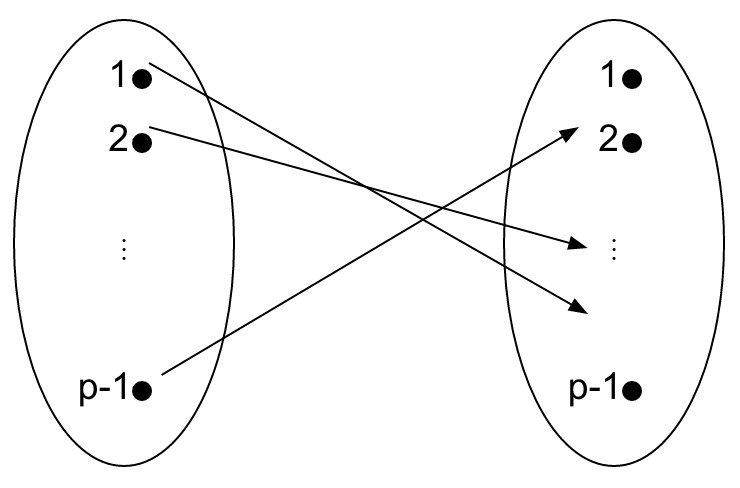
\includegraphics[width=4.5cm, height=30mm]{proof}
\end{center}
So if we multiply all elements in the domain together this should equal the product of all the elements in the image: \newline
\[ 1 * 2 * \dotsc * (p-1) \mod p \equiv (1a) * (2a) * \dotsc * ((p-1)a) \mod p\]
\[(p-1)! \mod p \equiv a^{p-1} * (p-1)! \mod p\]
\[1 \equiv a^{p-1} \mod p \]
\end{solution}

